\chapter{Figures And Charts}
\section{PLAXIS}
Plaxis2d file URL: \url{https://github.com/rdmorgnzation/soilbearing/blob/main/media/testdata/BHLog.plxzip}\\
\vfill
Start a new project with axisymmetry since it is for circular footing.
\begin{figure}[hbtp]
  \centering
  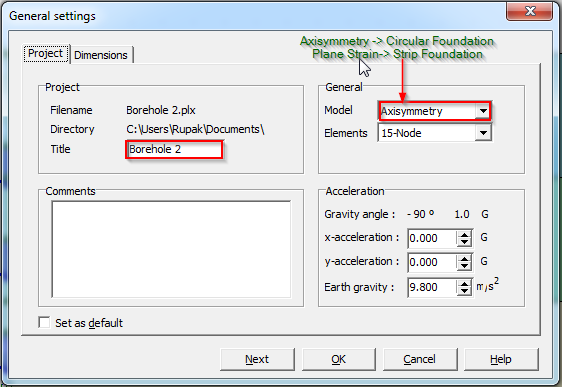
\includegraphics[height=0.33\textheight]{images/plx/a (1).png}
  \caption{Project Options}
  \vfill
  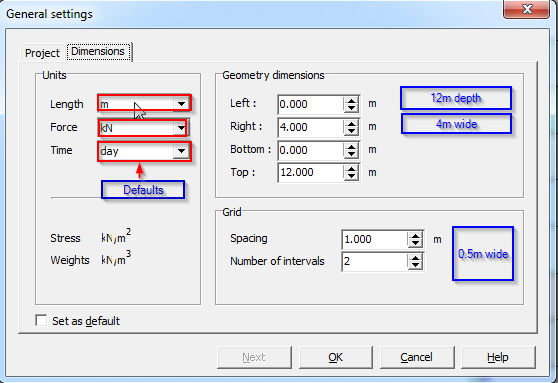
\includegraphics[height=0.33\textheight]{images/plx/a (2).png}
  \caption{Dimension Options}
\end{figure}
\vfill
\pagebreak

\begin{landscape}
\begin{figure}[hbtp]
  Create a new model for soil with displacements.
  \centering
  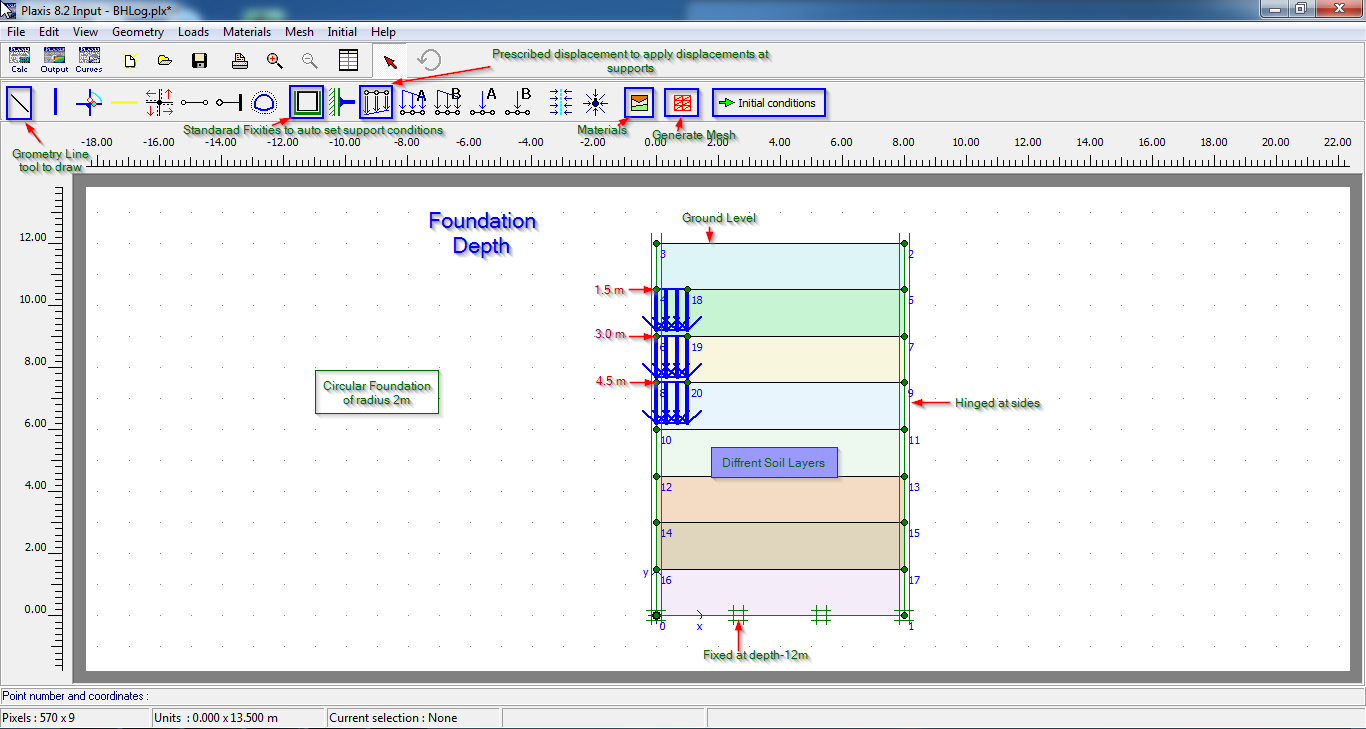
\includegraphics[width=0.9\linewidth, height=0.9\textheight,keepaspectratio]{images/plx/a (4).png}
  \caption{Main drawing page}
\end{figure}
\end{landscape}
\pagebreak

\begin{landscape}
\begin{figure}[hbtp]
  \centering
  \hfill
  \begin{minipage}[c]{0.4\linewidth}
  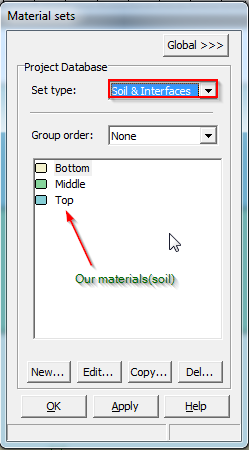
\includegraphics[width=\linewidth, height=0.9\textheight,keepaspectratio]{images/plx/a (3).png}
  \caption{Soil List(Materials)}
  \end{minipage}
  \hfill
  \begin{minipage}[c]{0.4\linewidth}
  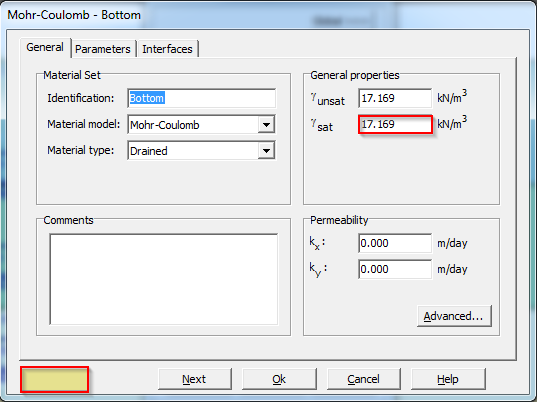
\includegraphics[width=\linewidth, height=0.4\textheight,keepaspectratio]{images/plx/a (6).png}
  \caption{General Soil Parameters}
  \vfill
  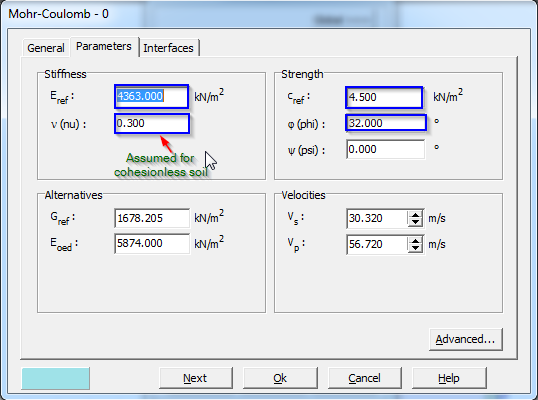
\includegraphics[width=\linewidth, height=0.4\textheight,keepaspectratio]{images/plx/a (7).png}
  \caption{Other Soil Parameters}
  \end{minipage}
  \hfill
  \begin{minipage}[c]{0.2\linewidth}
   Create materials as in the sample calculation.
  \end{minipage}
\end{figure}
\end{landscape}
\pagebreak

\begin{figure}[hbtp]
  \centering
  \vfill
  Generate Mesh
  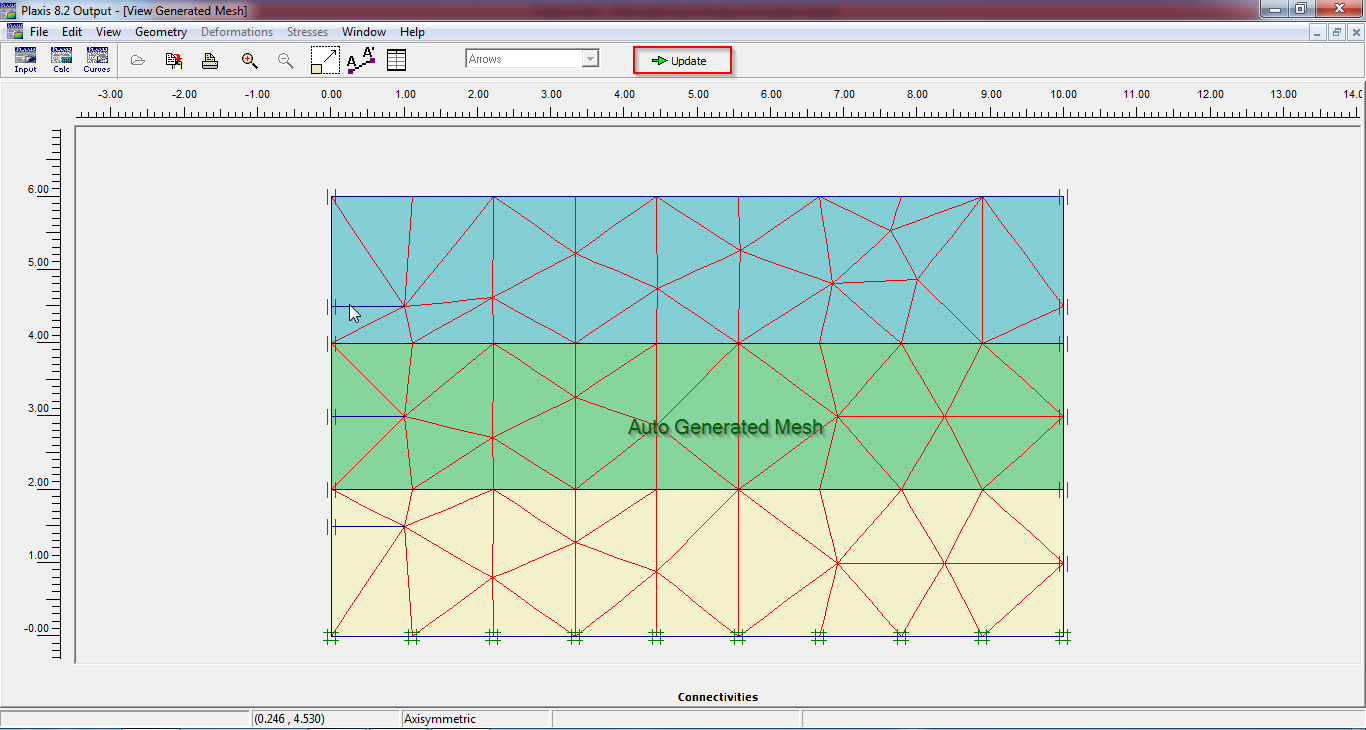
\includegraphics[width=\linewidth, height=0.4\textheight,keepaspectratio]{images/plx/a (5).png}
  \caption{Auto generated mesh}
  \vfill
  Go to initial conditions, and create ground water line.
  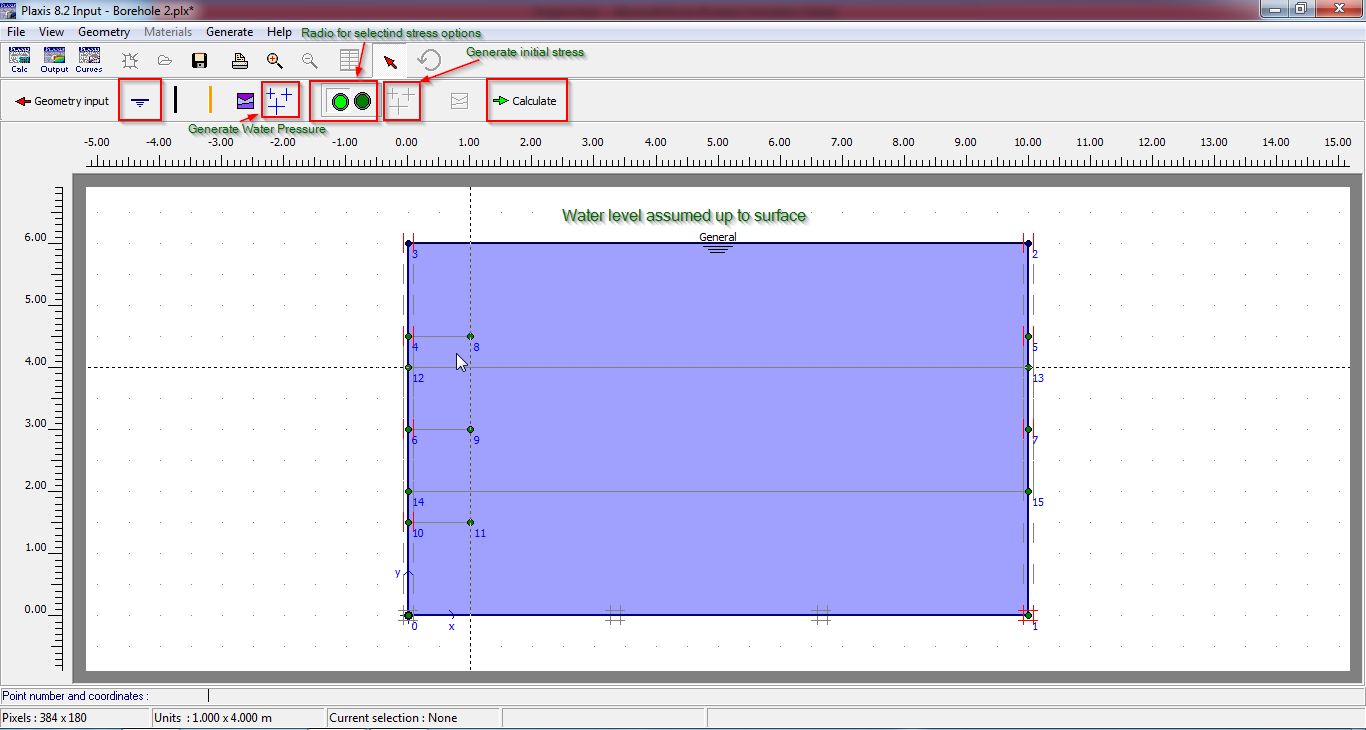
\includegraphics[width=\linewidth, height=0.4\textheight,keepaspectratio]{images/plx/a (8).png}
  \caption{Ground Water Options}
  \vfill
\end{figure}
\pagebreak

\begin{figure}[hbtp]
  \centering
  Go with default options.
  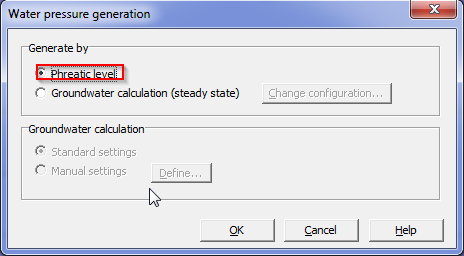
\includegraphics[height=0.25\textheight]{images/plx/a (9).png}
  \caption{Water pressure generation options}
  \vfill
  Generate pore water pressure.\\
  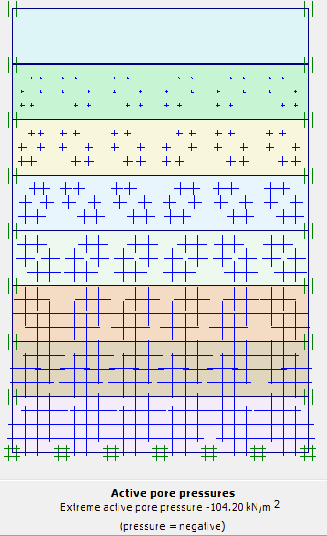
\includegraphics[height=0.45\textheight]{images/plx/a (10).png}
  \caption{Generated pore water pressures}
  Generate K0 stresses now, but in this sample it will be calculated later. Now go to calculation.
\end{figure}
\pagebreak

\begin{figure}[hbtp]
  \vfill
  \centering
  Create calulation steps as in fig.
  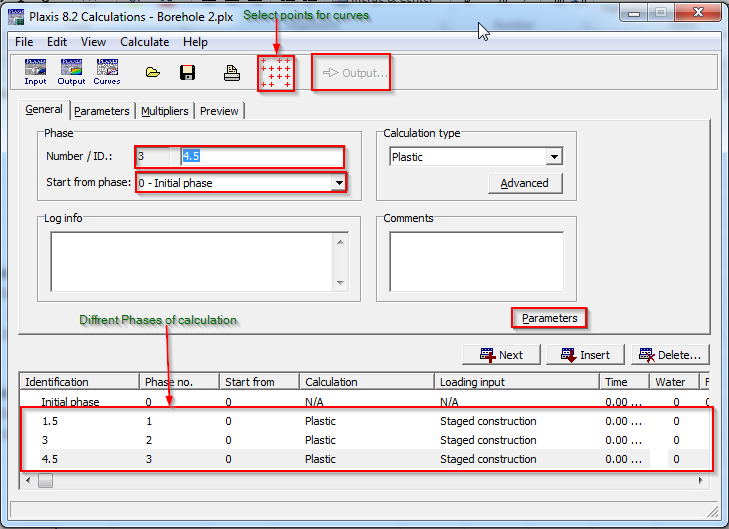
\includegraphics[height=0.4\textheight]{images/plx/a (13).png}
  \caption{Main calculation dialog}
  \vfill
  For calculating stress due to self wt, set up as follows.
  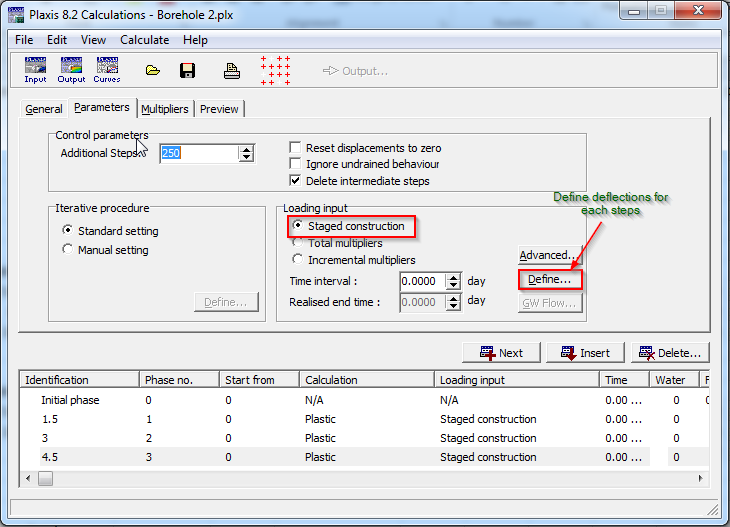
\includegraphics[height=0.4\textheight]{images/plx/a (14).png}
  \caption{Parameters tab}
  \vfill
\end{figure}
\pagebreak

\begin{landscape}
\begin{figure}[hbtp]
  \vfill
  \centering
  \begin{minipage}[c]{0.35\linewidth}
    \vfill
	Set MWeight to 1, ie. Self weight.
    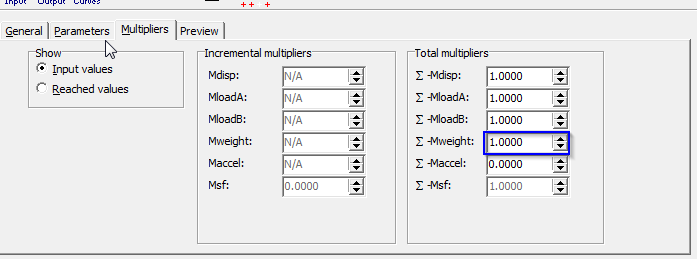
\includegraphics[width=\linewidth, height=0.7\textheight,keepaspectratio]{images/plx/a (15).png}
    \caption{Multipliers Dialog}
    \vfill
	Add new phases for capacity calculation.
    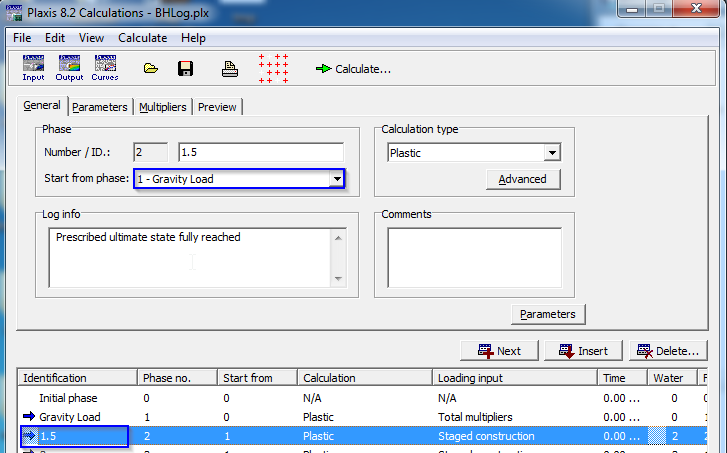
\includegraphics[width=\linewidth, height=0.3\textheight,keepaspectratio]{images/plx/a (16).png}
    \caption{New phase}
    \vfill
  \end{minipage}
  \hfill
  \begin{minipage}[c]{0.6\linewidth}
  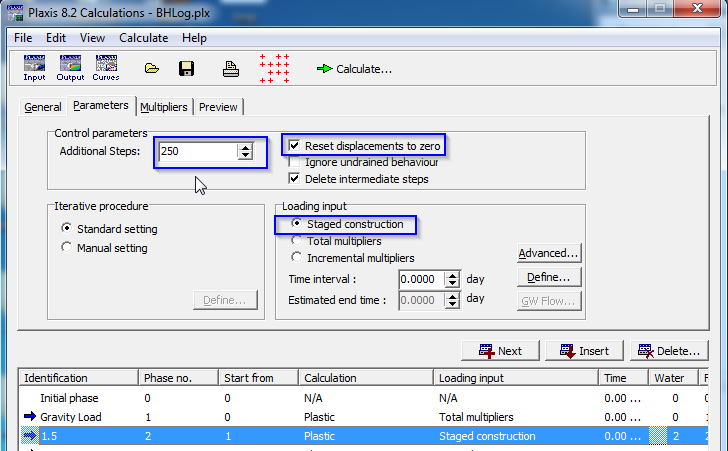
\includegraphics[width=\linewidth, height=0.8\textheight,keepaspectratio]{images/plx/a (17).png}
  \caption{Parameters for capacity}
  Set parameters.
  \end{minipage}
\vfill
\end{figure}
\end{landscape}
\pagebreak

\begin{landscape}
\begin{figure}[hbtp]
  \vfill
  \centering
  \begin{minipage}[c]{0.35\linewidth}
    \vfill
	Enable Displacement on required depth.
    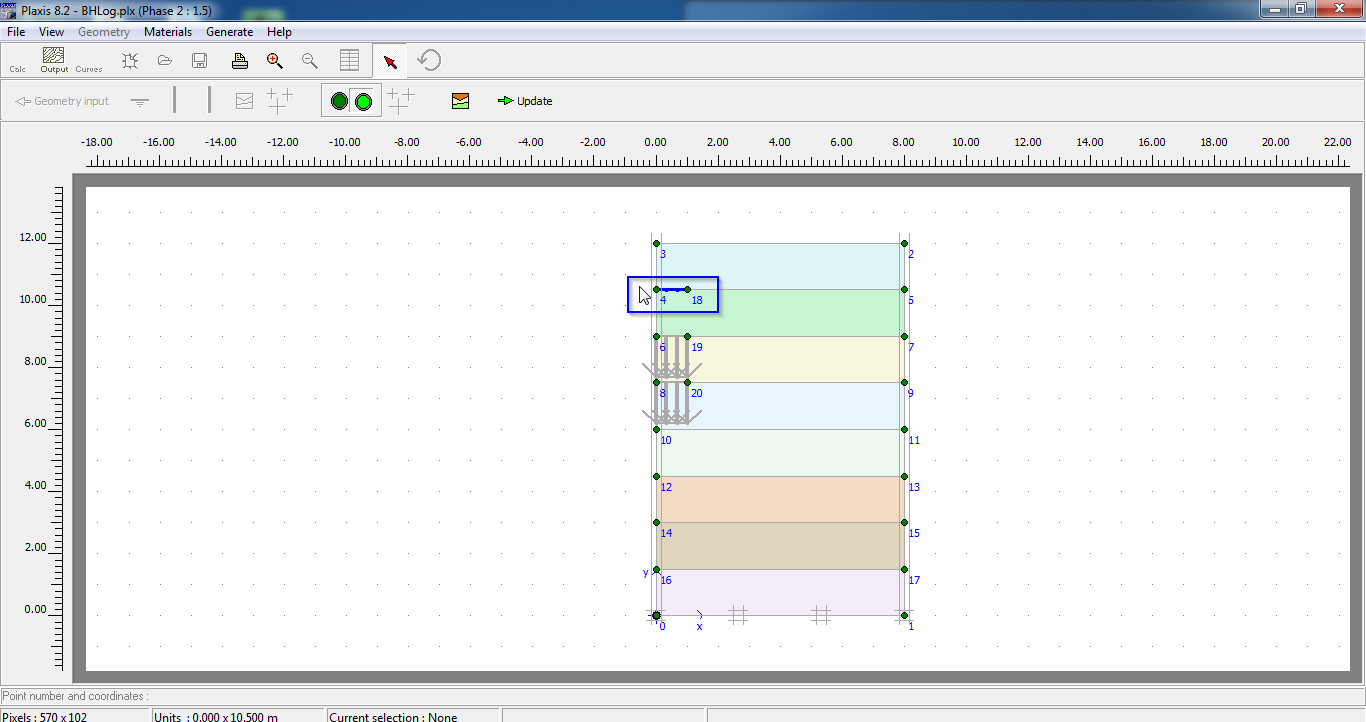
\includegraphics[width=\linewidth, height=0.7\textheight,keepaspectratio]{images/plx/a (18).png}
    \caption{Define Dialog}
    \vfill
	Double click to set displacement value.
    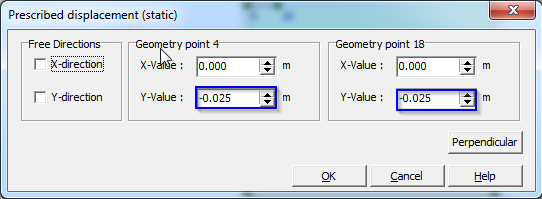
\includegraphics[width=\linewidth, height=0.3\textheight,keepaspectratio]{images/plx/a (19).png}
    \caption{Prescribed displacement dialog.}
    \vfill
  \end{minipage}
  \hfill
  \begin{minipage}[c]{0.6\linewidth}
  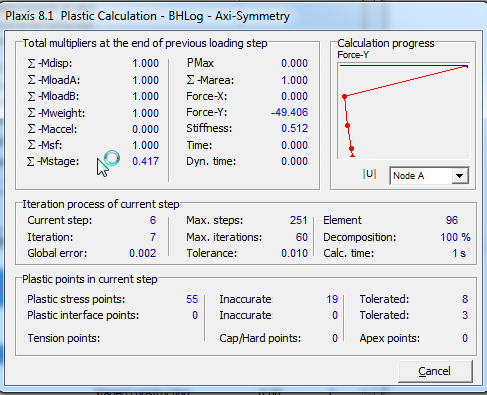
\includegraphics[width=\linewidth, height=0.8\textheight,keepaspectratio]{images/plx/a (20).png}
  \caption{Calculation Progress Dialog}
  After setting all up start calculation.
  \end{minipage}
\vfill
\end{figure}
\end{landscape}
\pagebreak

\begin{landscape}
\begin{figure}[hbtp]
  \vfill
  \begin{minipage}[c]{0.6\linewidth}
  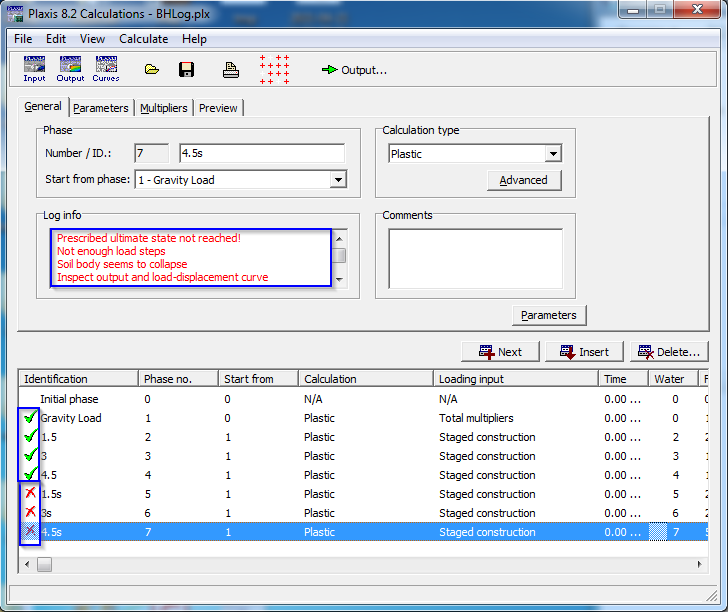
\includegraphics[width=\linewidth, height=0.8\textheight,keepaspectratio]{images/plx/a (21).png}
  \caption{Log file}
  This will not always work as the force will decrease (mostly in shear). If that is case check for output diagram. Here log as in figure is used which is saved in .LAV file.
  \end{minipage}
  \hfill
  \centering
  \begin{minipage}[c]{0.35\linewidth}
    \vfill
	Check results for capacity. For shear these should fail.
    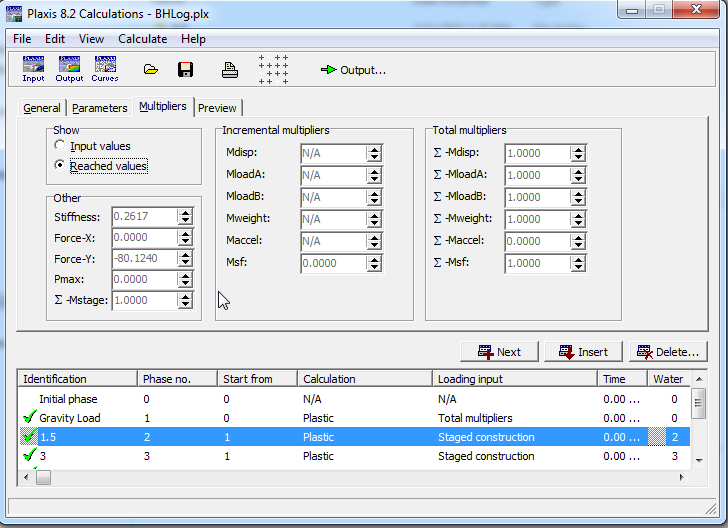
\includegraphics[width=\linewidth, height=0.7\textheight,keepaspectratio]{images/plx/a (22).png}
    \caption{Calculation dialog after calculation is complete.}
    \vfill
	Check multipliers \textgreater Reached Values \textgreater Force-Y.
    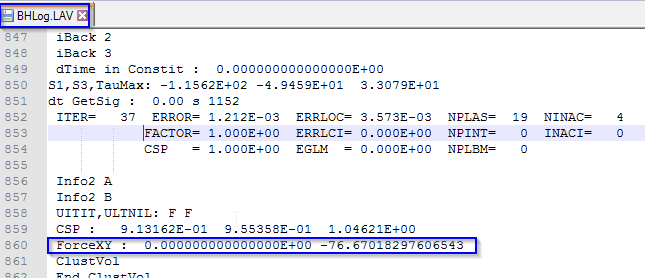
\includegraphics[width=\linewidth, height=0.3\textheight,keepaspectratio]{images/plx/a (23).png}
    \caption{Prescribed displacement dialog.}
	Here our result is -80.1240. So our capacity is $ 80.1240 * 2 \pi / (\pi * 2^2) = 40.062kN/m^2$ for 1.5m displacement.
    \vfill
  \end{minipage}
\vfill
\end{figure}
\end{landscape}
\pagebreak

\begin{landscape}
\section{GIS}
\begin{figure}[hbtp]
  \centering
  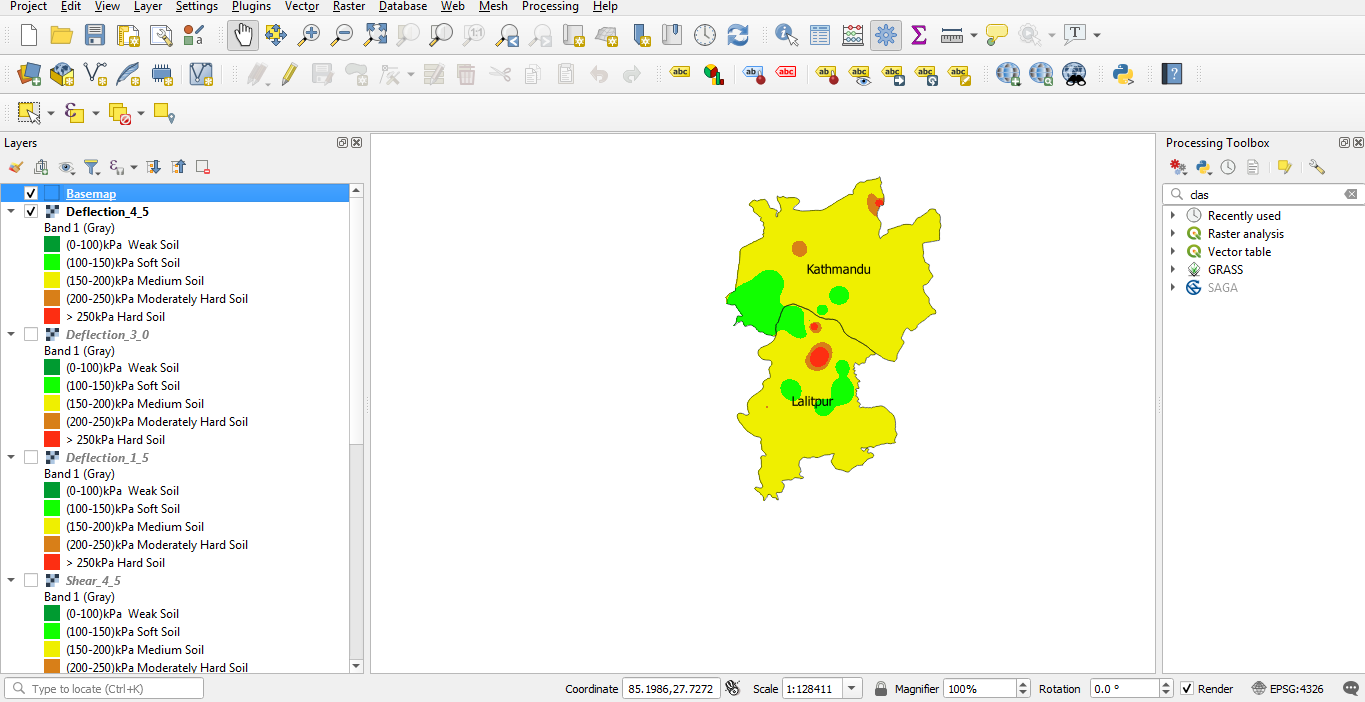
\includegraphics[width=0.8\linewidth, height=0.8\textheight,keepaspectratio]{images/gis/Screenshot (1).png}
  \caption{GIS Main Screen}
\end{figure}
\end{landscape}
\pagebreak
\begin{landscape}
\begin{figure}[hbtp]
  \centering
  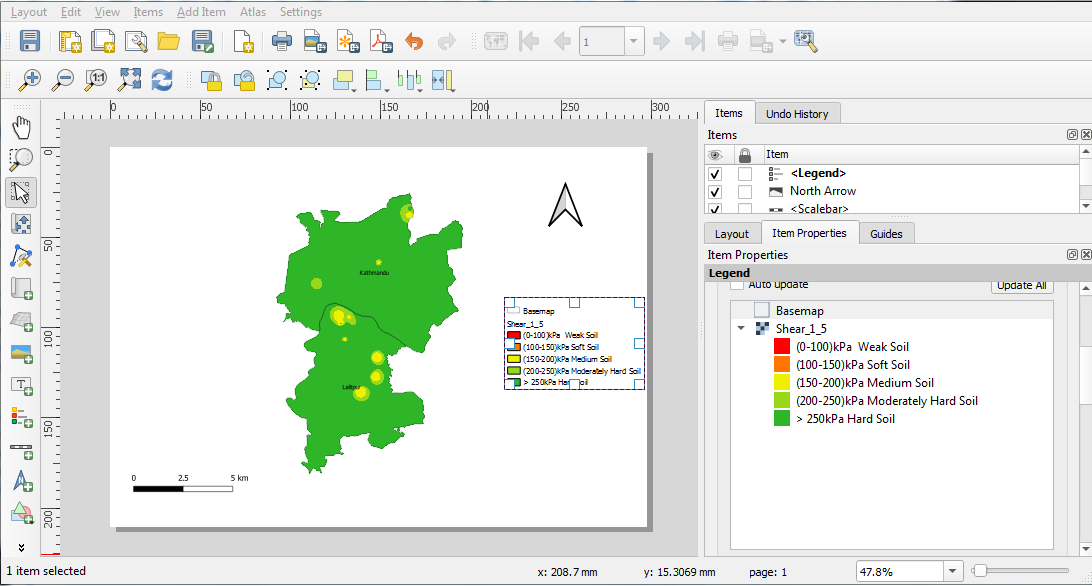
\includegraphics[width=\linewidth, height=\textheight,keepaspectratio]{images/gis/Screenshot (2).png}
  \caption{GIS Map Layout}
\end{figure}
\end{landscape}
\pagebreak

\begin{figure}[hbtp]
  \centering
  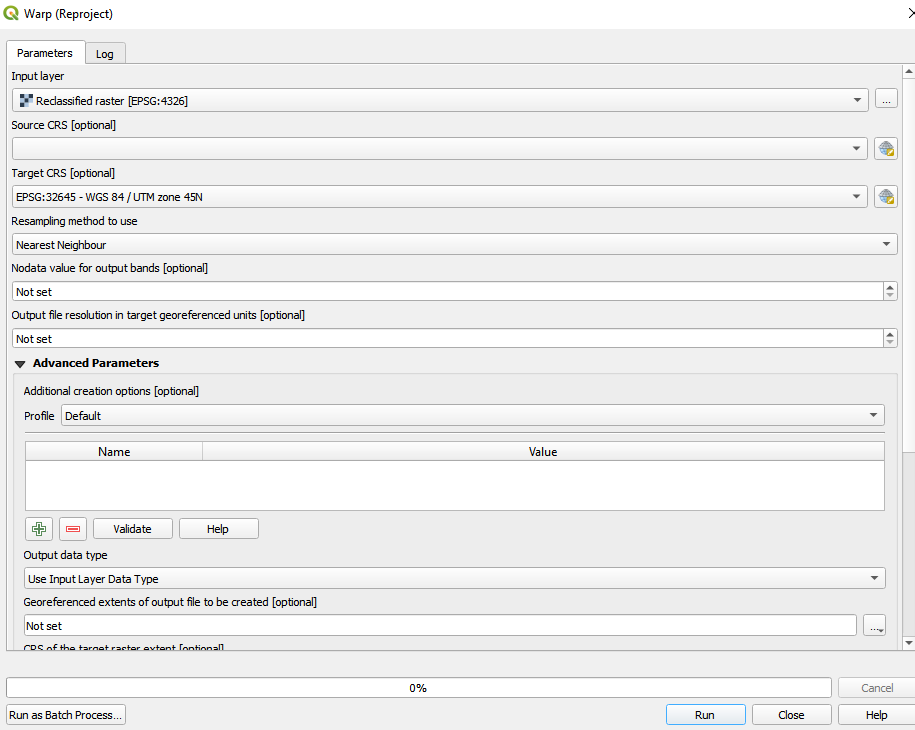
\includegraphics[height=0.33\textheight]{images/gis/Warp to UTM.png}
  \caption{Wrap Projection}
  \vfill
  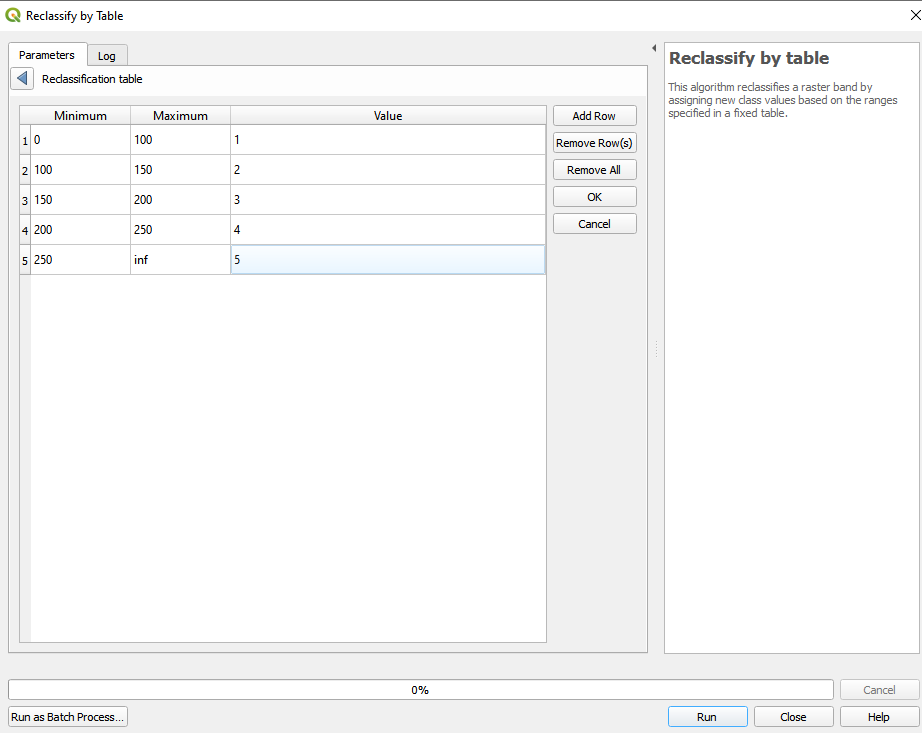
\includegraphics[height=0.33\textheight]{images/gis/Reclassify.png}
  \caption{Reclassify by table tool}
\end{figure}
\pagebreak

\begin{figure}[hbtp]
  \centering
  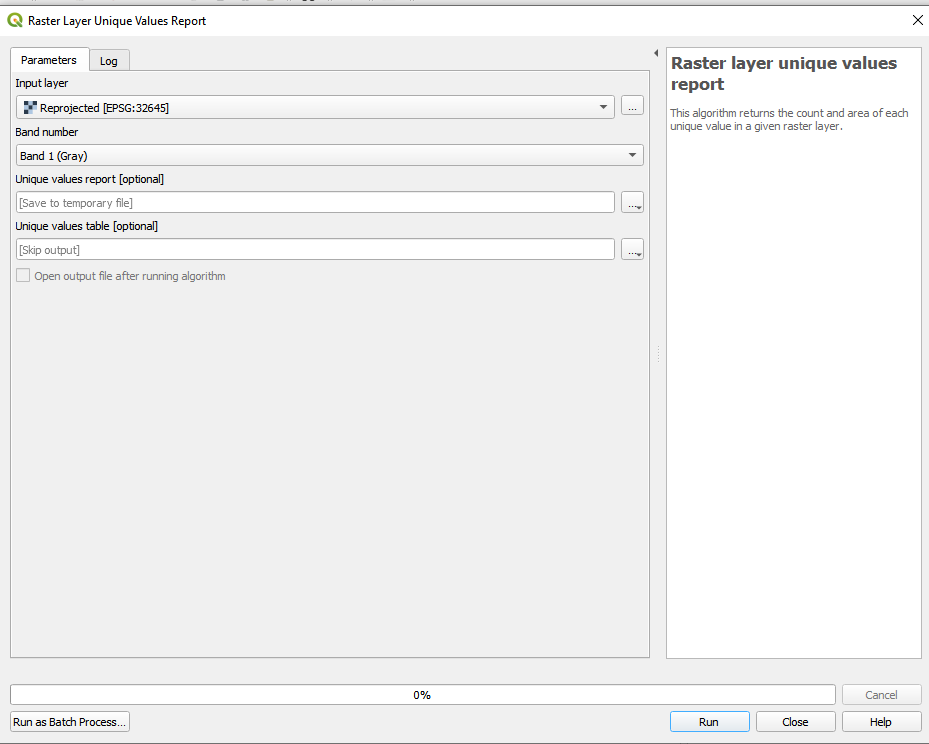
\includegraphics[height=0.33\textheight]{images/gis/Report.png}
  \caption{Report Tool}
  \vfill
  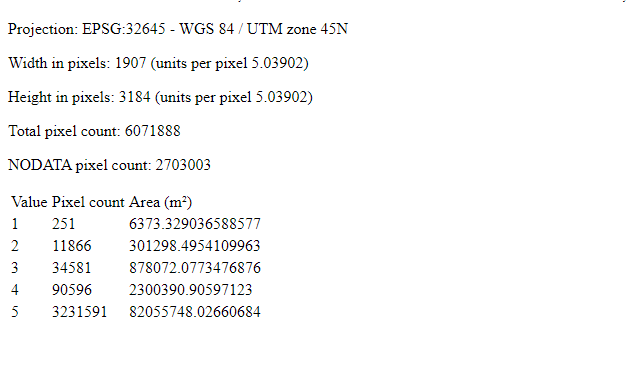
\includegraphics[height=0.33\textheight]{images/gis/AreaSumReport.png}
  \caption{Result From Report}
\end{figure}
\pagebreak